%!TEX root = /Users/stefano/Documents/Bonsai Club/TWBC/twbc.tex

\headline{{\textbf{\Large\sffamily TWBC Workshops:}}\\
          {\textbf{\large\sffamily Air\--Layering Bonsai}}}
\label{2025-05-layers}
\noindent
Our club's latest hands\--on session saw Steve back in action, this time tackling \textit{air\--layering} --- the perfect follow\--up to his grafting workshop! True to form, he encouraged everyone to bring along their own trees for some practical work. And just like last time, we all gathered round as Steve demonstrated each step on his own tree, while guiding members through their attempts.

Below you'll find all the key points covered --- from the theory behind air\--layering to a step\--by\--step recap of the practical session. Whether you attended or missed out, this guide will help you master this incredibly useful technique!

\begin{window}[2,l,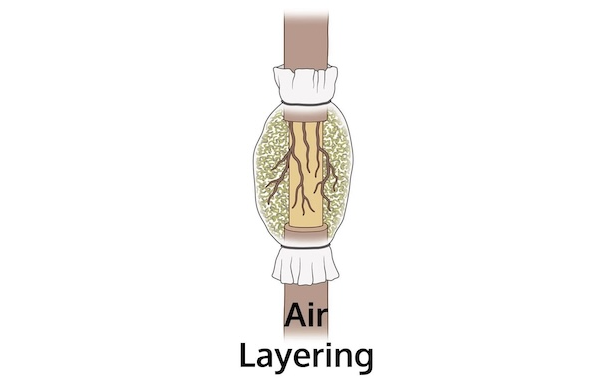
\includegraphics[width=1.0\columnwidth]{2025_05/res/air-layering.png},\centerline{\emph{A diagram with a cut\--out view of an air\--layer.}}]
\end{window}

\medskip
\topic{What is It and Why Should You Do It??}
\noindent
Air\--layering is a propagation method where we encourage roots to grow on a branch or trunk while it's still attached to the parent tree. Once the roots are established, we separate the new plant, giving us a second bonsai (or a better \textit{nebari} on the original one).  

There are plenty of great reasons to try air\--layering---whether you're looking to improve your bonsai's design, rescue an awkward branch, or even grow a whole new tree! Some of the key benefits include:

\begin{itemize}
    \item \textbf{Improving Nebari} --- Remove ugly roots or create a better base.  

    \item \textbf{Shortening a Trunk} --- Turn a leggy tree into a more compact bonsai.  

    \item \textbf{Salvaging a Bad Design} --- If the lower branches are weak but the top is great, air\--layer the top!  

    \item \textbf{Propagation} --- Clone your favourite tree for free.  

    \item \textbf{Correcting Taper Issues} --- Thick upper trunk? Air\--layer to create better\--proportioned trees.  
\end{itemize}

\columnbreak

\begin{figure*}[!t]
\centering
\begin{minipage}[b]{.30\textwidth}
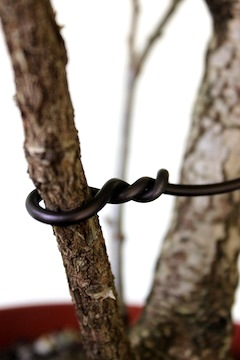
\includegraphics[angle=0,origin=c,width=1.0\textwidth]{2025_05/res/air-layer-tourniquet.JPG}
\end{minipage}\qquad
\begin{minipage}[b]{.30\textwidth}
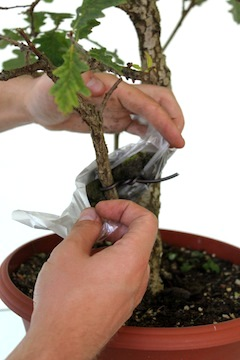
\includegraphics[angle=0,origin=c,width=1.0\textwidth]{2025_05/res/air-layer-moss.JPG}
\end{minipage}\qquad
\begin{minipage}[b]{.30\textwidth}
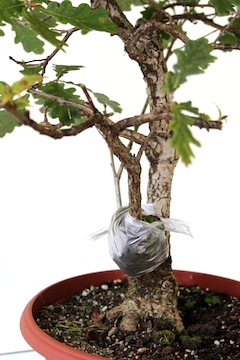
\includegraphics[angle=0,origin=c,width=1.0\textwidth]{2025_05/res/air-layer-finished.JPG}
\end{minipage}
\medskip 

\centerline{%
\emph{The Tourniquet method applied to on a Oak specimen.}}
\end{figure*}

\medskip
\topic{Air\--Layering vs. Ground\--Layering}
\noindent
A similar technique to air\--layering is \textbf{ground\--layering}, where propagation happens while the branch remains attached to the parent tree---but instead of roots forming in a moss\--wrapped bundle in mid\--air, the process occurs underground. In ground\--layering, a flexible low branch is bent down, partially buried in soil, and wounded to trigger root growth at the buried section. 

Both methods allow the new plant to draw nutrients from the parent while developing its own roots, making them more reliable than cuttings. However, air\--layering offers greater control, especially in bonsai, since it works on thick trunks and high branches that can't be bent into the soil. Ground\--layering is simpler but limited to flexible, low\--growing material---ideal for garden shrubs like willows or cotoneasters. 

For bonsai, air\--layering is often preferred because it lets us target specific sections of the tree and shape the new root system precisely.

\medskip
\topic{Before You Start: Is Your Tree Ready?}
\noindent
Not every tree is a good candidate for air\--layering. To begin with, not every tree plays nicely with air\--layering---some species root like champions while others need more convincing! 
If you're working with any of these cooperative varieties, you're in luck:

\begin{itemize}
    \item \textbf{Ficus} --- Almost foolproof, great for beginners. 

    \item \textbf{Elms} (\textit{Zelkova}, \textit{Chinese Elm}) --- Respond very well.

    \item \textbf{Maples} (\textit{Acer palmatum}) --- Wait until the new leaves have hardened off (about a month after budding).  
    
    \item \textbf{Pines \& Junipers} --- Possible but trickier; best left to more experienced members.
\end{itemize}

Now, just because your tree can be air\--layered doesn't always mean it should be --- there are times when even the most tempting branch should be left alone! 
Here's what to consider:  

\begin{itemize}
    \item \textbf{Recently Repotted Trees} --- If your tree is still recovering, wait at least a full growing season.

    \item \textbf{Weak or Unhealthy Trees} --- Air\--layering is stressful; only strong, vigorous trees should undergo it.

    \item \textbf{Wrong Season} --- Most trees air\--layer best in \textit{late spring to early summer} (May\--July in the UK), when the sap is flowing strongly and the temperatures are in 15\--25 Celsius. 
\end{itemize}

As Steve explained during the workshop while preparing his tools: \textit{``If you're unsure whether your tree is ready, don't hesitate to ask. That's what these sessions are for -- so that members can help each other out. Just keep in mind, species matters. While maples might show roots in 8\--12 weeks, pines can take a full year or more.''}

(He's not kidding: ask anyone who's tried layering pines---it's a marathon, not a sprint!)
\columnbreak

\medskip
\topic{The Step by Step Air\--Layering Process}
\noindent
Before diving in, it's always good to get the toolkit sorted. You'll want to have these essentials on hand (no need to stress if you're missing a particular tool: a good pair of secateurs will handle most of the job, and fellow members are usually happy to share their specialized equipment or spares if needed):

\begin{itemize}
    \item \textbf{Sharp knife} (or grafting knife)  

    \item \textbf{Sphagnum moss} (soaked in water)  

    \item \textbf{Rooting hormone} (powder or gel)  

    \item \textbf{Clear plastic wrap} or \textbf{foil} (or both)

    \item \textbf{Wire} (or zip ties)  

    \item \textbf{A pot} or \textbf{plastic bag} (optional) 
\end{itemize}

As Steve remarked during the workshop, \textit{``Once you've got everything prepared --- moss soaked, knife sharp, and your tree selected --- we can begin the actual process. I'll demonstrate each step carefully so you can follow along now or refer back later.''}

\begin{figure*}[!t]
\centering
\begin{minipage}[b]{.30\textwidth}
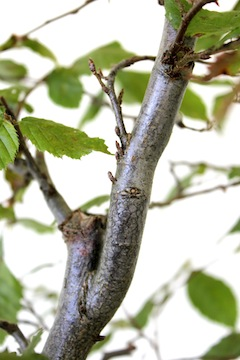
\includegraphics[angle=0,origin=c,width=1.0\textwidth]{2025_05/res/air-layer-ring.JPG}
\end{minipage}\qquad
\begin{minipage}[b]{.30\textwidth}
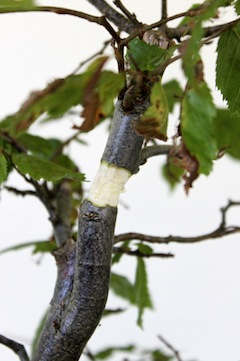
\includegraphics[angle=0,origin=c,width=1.0\textwidth]{2025_05/res/air-layer-ring2.JPG}
\end{minipage}\qquad
\begin{minipage}[b]{.30\textwidth}
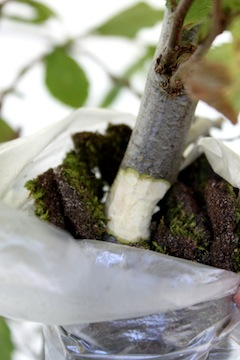
\includegraphics[angle=0,origin=c,width=1.0\textwidth]{2025_05/res/air-layer-ring3.JPG}
\end{minipage}
\medskip 

\centerline{%
\emph{The Ring Bark method demonstrated on a Hornbeam.}}
\end{figure*}

\begin{itemize}
    \item \textbf{Step 1.} \textit{Choosing the Right Spot}
    \begin{itemize}
        \item Look for a healthy branch or trunk section with good taper.
        
        \item Avoid nodes (knobbly bits where branches emerge) as they can complicate rooting.

        \item If you want to keep the parent tree alive, make sure to have at least a healthy branch below the air\--layer.
    \end{itemize}

    \item \textbf{Step 2.} \textit{Making the Cut}
    \begin{itemize}
        \item \textbf{Option 1:} \textit{Simple Ring Barking}
        \begin{itemize}
            \item[\tiny$\blacksquare$] Make \textbf{two parallel cuts} around the branch (about 1\--1.5x the diameter apart).
        
            \item[\tiny$\blacksquare$] Remove the bark and cambium (green layer) between them, leaving bare wood.
        \end{itemize}

        \item \textbf{Option 2:} \textit{Tourniquet Method (Advanced, for stubborn species)}
        \begin{itemize}
            \item[\tiny$\blacksquare$] Wrap wire tightly around the branch.
        
            \item[\tiny$\blacksquare$] Over time, it will cut into the bark, forcing root growth above it.
        \end{itemize}
    \end{itemize}
    %
    During the workshop, Steve demonstrated the importance of removing all cambium, tapping his knife lightly on the branch to emphasize the point. \textit{``This step is critical,''} he explained. \textit{``You need to thoroughly scrape the exposed wood --- any remaining cambium will let the tree heal over the wound, undoing all your work.''}

    \item \textbf{Step 3.} \textit{Applying Rooting Hormone}
    \begin{itemize}
        \item Dust the \textbf{top edge} of the cut (where roots will emerge) with hormone powder.
        
        \item Avoid getting it on the lower part (we don't want roots growing downward from the top of the mother tree).
    \end{itemize}

    \item \textbf{Step 4.} \textit{Wrapping with Moss}
    \begin{itemize}
        \item \textbf{\textit{Why sphagnum moss?}} It holds moisture, is slightly acidic (discourages rot), and allows air flow. 
        
        \item Squeeze out excess water and pack it around the cut. 

        \item Wrap tightly in \textbf{clear plastic} (lets you monitor roots) or \textbf{foil} (keeps it darker, which some species prefer). If unsure, research your species recommendations online or use the foil over the clear plastic.

        \item Secure with wire or zip ties---\textbf{don't let it dry out!}
    \end{itemize}
    %
    Steve explained an alternative to plastic wrap during the workshop. \textit{``If you prefer using a pot,''} he said, \textit{``split it and secure it on the branch around the cut, then fill it with a mix of sphagnum moss and akadama in equal parts --- it will function like a miniature greenhouse for the developing roots.''}

    \item \textbf{Step 5.} \textit{Watering \& Maintenance}
    \begin{itemize}
        \item Check moisture weekly: \textbf{damp, not soggy!} 

        \item If it dries out, inject water for instance with a syringe.

        \item If too wet, loosen the wrap slightly to allow airflow.
    \end{itemize}
\end{itemize}

\medskip
\topic{Aftercare: Waiting for Roots}
\noindent
The work isn't over once you've wrapped the moss---now comes the observation phase. Air layers can take weeks or even months to root, and what you find when you check will determine your next steps. Some will develop strong roots quickly, others may need more time, and a few might not take at all.

Here's what to watch for, how long to wait, and what to do in each scenario.

\begin{itemize}
    \item \textbf{How Long Until Roots Appear?}
    \begin{itemize}
        \item \textbf{Maples, Elms, Ficus:} 8\--12 weeks  

        \item \textbf{Pines, Junipers:} 6 months\--1 year (patience needed!)
    \end{itemize}

    \item \textbf{When to Separate?}
    \begin{itemize}
        \item Wait until you see \textbf{a good network of white roots} (not just one or two).

        \item Cut \textit{below the new roots} and pot the new tree in \textbf{well\--draining soil}.
    \end{itemize}

    \item \textbf{If It Fails?}
    \begin{itemize}
        \item \textbf{Callusing (no roots)?} You can try again next season. 

        \item \textbf{Dead top?} Just remove it---the parent tree will bounce back.
    \end{itemize}

    \item \textbf{After Separation Care:}
    \begin{itemize}
        \item Keep the new tree in \textbf{dappled shade} for a few weeks.

        \item Mist foliage to reduce stress.

        \item \textbf{No fertiliser} until you see strong new growth.
    \end{itemize}
\end{itemize}

Steve summed it up plainly: \textit{``Give it time. Roots develop at their own pace --- when you check and see nothing, resist the urge to cut. Another two weeks won't hurt, but separating too early certainly will.''}

\begin{center}
    $\cdots$
\end{center}

\noindent
We hope this guide serves as a useful reference for practising air\--layering, whether you're replicating what you learned at the workshop or trying it for the first time. If you have questions, don't hesitate to ask Steve or other TWBC members---you'll find us at meetings or on the club's WhatsApp group.

Best of luck with your layers!

\closearticle
\columnbreak
